% Springer Nature journal template Version 3.1, December 2024.
% Working bibliography style; change it to match the selected journal.
\documentclass[pdflatex,sn-basic,Numbered]{sn-jnl}

\usepackage{graphicx}
\usepackage{multirow}
\usepackage{amsmath,amssymb,amsfonts}
\usepackage{xcolor}
\usepackage{booktabs}
\usepackage{tabularx}
\usepackage{listings}
\usepackage{tikz}
\usepackage{pgfplots}
\usepackage{microtype}
\usepackage{placeins}
\usepackage{capt-of}
\usetikzlibrary{arrows.meta,backgrounds,calc,fit,matrix,positioning,shapes.geometric}
\pgfplotsset{compat=1.18}

\definecolor{bpblue}{HTML}{2563EB}
\definecolor{bpgreen}{HTML}{059669}
\definecolor{bporange}{HTML}{D97706}
\definecolor{bpred}{HTML}{DC2626}
\definecolor{bpink}{HTML}{EEF2FF}
\definecolor{bpgray}{HTML}{475569}
\tikzset{
  box/.style={draw=bpgray, rounded corners=2pt, fill=white, align=center,
    minimum height=8mm, inner sep=4pt, font=\small},
  layer/.style={box, minimum width=32mm},
  flow/.style={-Latex, semithick, draw=bpgray},
  optional/.style={flow, dashed},
  note/.style={font=\scriptsize, align=center, text=bpgray}
}
\lstset{basicstyle=\ttfamily\small, frame=single, breaklines=true,
  keywordstyle=\color{bpblue}, commentstyle=\color{bpgray}, showstringspaces=false}

% Generated by paper/artifact/summarize-study.ts; do not edit manually.
\newcommand{\ApiCount}{505}
\newcommand{\ArqueroCases}{82}
\newcommand{\ArqueroWins}{72}
\newcommand{\ArqueroGeoSpeedup}{2.15}
\newcommand{\GroupbyGeoSpeedup}{1.28}
\newcommand{\SortGeoSpeedup}{1.93}
\newcommand{\CountsGeoSpeedup}{4.54}
\newcommand{\MergeGeoSpeedup}{0.34}
\newcommand{\PandasCases}{10}
\newcommand{\PandasWins}{6}
\newcommand{\PandasGeoSpeedup}{1.44}
\newcommand{\WasmSortMin}{1.75}
\newcommand{\WasmSortMax}{2.05}
\newcommand{\WasmFilterMin}{0.23}
\newcommand{\WasmFilterMax}{0.30}
\newcommand{\FreshProcesses}{720}
\newcommand{\FreshIterations}{14,400}
\newcommand{\ConformanceCases}{2,500}
\newcommand{\ConformancePasses}{2,500}
\newcommand{\ConformancePercent}{100.00}
\newcommand{\BackendCases}{2,500}
\newcommand{\BackendPasses}{2,500}
\newcommand{\NpmTarballKiB}{130.7}
\newcommand{\NpmUnpackedKiB}{546.1}
\newcommand{\NpmEntryCount}{77}
\newcommand{\CoreBundleKiB}{180.2}
\newcommand{\CoreBundleGzipKiB}{51.6}
\newcommand{\WasmBytes}{7,359}
\newcommand{\BrowserBundleBytes}{2,683}
\newcommand{\BrowserBundleGzipBytes}{996}
\newcommand{\BrowserBundleBrotliBytes}{877}
\newcommand{\WasmGzipBytes}{2,984}
\newcommand{\WasmBrotliBytes}{2,614}

% Generated by paper/artifact/summarize-expanded-study.ts; do not edit manually.
\newcommand{\CompetitorProcesses}{400}
\newcommand{\CompetitorIterations}{4,000}
\newcommand{\CompetitorCells}{16}
\newcommand{\PublicProcesses}{200}
\newcommand{\PublicIterations}{2,000}
\newcommand{\PublicCells}{8}
\newcommand{\BrowserContexts}{180}
\newcommand{\BrowserTimedCalls}{10,800}
\newcommand{\GroupBunPandaOpMs}{2.67}
\newcommand{\GroupBunPandaLoadMs}{6.96}
\newcommand{\GroupArqueroOpMs}{4.22}
\newcommand{\GroupArqueroLoadMs}{4.73}
\newcommand{\GroupDanfoOpMs}{16.08}
\newcommand{\GroupDanfoLoadMs}{19.99}
\newcommand{\GroupPolarsOpMs}{1.59}
\newcommand{\GroupPolarsLoadMs}{6.72}
\newcommand{\GroupDuckDBOpMs}{3.06}
\newcommand{\GroupDuckDBLoadMs}{119.27}
\newcommand{\FilterBunPandaOpMs}{2.05}
\newcommand{\FilterBunPandaLoadMs}{6.44}
\newcommand{\FilterArqueroOpMs}{6.60}
\newcommand{\FilterArqueroLoadMs}{6.48}
\newcommand{\FilterDanfoOpMs}{114.55}
\newcommand{\FilterDanfoLoadMs}{105.85}
\newcommand{\FilterPolarsOpMs}{1.56}
\newcommand{\FilterPolarsLoadMs}{6.98}
\newcommand{\FilterDuckDBOpMs}{6.31}
\newcommand{\FilterDuckDBLoadMs}{123.86}
\newcommand{\CountsBunPandaOpMs}{0.68}
\newcommand{\CountsBunPandaLoadMs}{4.93}
\newcommand{\CountsArqueroOpMs}{2.83}
\newcommand{\CountsArqueroLoadMs}{3.84}
\newcommand{\CountsDanfoOpMs}{15.97}
\newcommand{\CountsDanfoLoadMs}{19.92}
\newcommand{\CountsPolarsOpMs}{1.62}
\newcommand{\CountsPolarsLoadMs}{6.53}
\newcommand{\CountsDuckDBOpMs}{3.09}
\newcommand{\CountsDuckDBLoadMs}{117.98}
\newcommand{\JoinBunPandaOpMs}{24.56}
\newcommand{\JoinBunPandaLoadMs}{26.39}
\newcommand{\JoinArqueroOpMs}{8.16}
\newcommand{\JoinArqueroLoadMs}{7.68}
\newcommand{\JoinDanfoOpMs}{1807.97}
\newcommand{\JoinDanfoLoadMs}{2359.89}
\newcommand{\JoinPolarsOpMs}{6.09}
\newcommand{\JoinPolarsLoadMs}{13.38}
\newcommand{\JoinDuckDBOpMs}{9.46}
\newcommand{\JoinDuckDBLoadMs}{126.10}
\newcommand{\PublicGroupBunPandaOpMs}{32.81}
\newcommand{\PublicGroupBunPandaLoadMs}{38.93}
\newcommand{\PublicGroupArqueroOpMs}{29.96}
\newcommand{\PublicGroupArqueroLoadMs}{29.55}
\newcommand{\PublicGroupDanfoOpMs}{65.54}
\newcommand{\PublicGroupDanfoLoadMs}{66.18}
\newcommand{\PublicGroupPolarsOpMs}{5.20}
\newcommand{\PublicGroupPolarsLoadMs}{14.60}
\newcommand{\PublicGroupDuckDBOpMs}{19.24}
\newcommand{\PublicGroupDuckDBLoadMs}{356.71}
\newcommand{\PublicFilterBunPandaOpMs}{5.75}
\newcommand{\PublicFilterBunPandaLoadMs}{38.65}
\newcommand{\PublicFilterArqueroOpMs}{14.23}
\newcommand{\PublicFilterArqueroLoadMs}{27.16}
\newcommand{\PublicFilterDanfoOpMs}{296.70}
\newcommand{\PublicFilterDanfoLoadMs}{265.00}
\newcommand{\PublicFilterPolarsOpMs}{2.70}
\newcommand{\PublicFilterPolarsLoadMs}{85.53}
\newcommand{\PublicFilterDuckDBOpMs}{10.71}
\newcommand{\PublicFilterDuckDBLoadMs}{446.16}
\newcommand{\PublicCountsBunPandaOpMs}{9.14}
\newcommand{\PublicCountsBunPandaLoadMs}{23.46}
\newcommand{\PublicCountsArqueroOpMs}{24.55}
\newcommand{\PublicCountsArqueroLoadMs}{30.58}
\newcommand{\PublicCountsDanfoOpMs}{79.52}
\newcommand{\PublicCountsDanfoLoadMs}{68.55}
\newcommand{\PublicCountsPolarsOpMs}{6.54}
\newcommand{\PublicCountsPolarsLoadMs}{68.15}
\newcommand{\PublicCountsDuckDBOpMs}{28.68}
\newcommand{\PublicCountsDuckDBLoadMs}{490.38}
\newcommand{\PublicJoinBunPandaOpMs}{120.00}
\newcommand{\PublicJoinBunPandaLoadMs}{150.35}
\newcommand{\PublicJoinArqueroOpMs}{27.80}
\newcommand{\PublicJoinArqueroLoadMs}{30.64}
\newcommand{\PublicJoinDanfoOpMs}{4496.54}
\newcommand{\PublicJoinDanfoLoadMs}{4360.63}
\newcommand{\PublicJoinPolarsOpMs}{66.98}
\newcommand{\PublicJoinPolarsLoadMs}{51.95}
\newcommand{\PublicJoinDuckDBOpMs}{29.30}
\newcommand{\PublicJoinDuckDBLoadMs}{483.13}
\newcommand{\ChromiumVersion}{151.0.7922.34}
\newcommand{\ChromiumInitMs}{4.75}
\newcommand{\ChromiumSortSpeedup}{1.78}
\newcommand{\ChromiumSortLower}{1.62}
\newcommand{\ChromiumSortUpper}{2.09}
\newcommand{\ChromiumFilterSpeedup}{1.63}
\newcommand{\ChromiumFilterLower}{1.42}
\newcommand{\ChromiumFilterUpper}{2.10}
\newcommand{\ChromiumGroupSpeedup}{2.63}
\newcommand{\ChromiumGroupLower}{2.20}
\newcommand{\ChromiumGroupUpper}{3.05}
\newcommand{\FirefoxVersion}{153.0}
\newcommand{\FirefoxInitMs}{46.21}
\newcommand{\FirefoxSortSpeedup}{0.47}
\newcommand{\FirefoxSortLower}{0.42}
\newcommand{\FirefoxSortUpper}{0.49}
\newcommand{\FirefoxFilterSpeedup}{0.59}
\newcommand{\FirefoxFilterLower}{0.50}
\newcommand{\FirefoxFilterUpper}{0.68}
\newcommand{\FirefoxGroupSpeedup}{0.08}
\newcommand{\FirefoxGroupLower}{0.07}
\newcommand{\FirefoxGroupUpper}{0.09}
\newcommand{\WebkitVersion}{26.5}
\newcommand{\WebkitInitMs}{9.14}
\newcommand{\WebkitSortSpeedup}{1.28}
\newcommand{\WebkitSortLower}{1.18}
\newcommand{\WebkitSortUpper}{1.52}
\newcommand{\WebkitFilterSpeedup}{1.19}
\newcommand{\WebkitFilterLower}{0.95}
\newcommand{\WebkitFilterUpper}{1.31}
\newcommand{\WebkitGroupSpeedup}{0.38}
\newcommand{\WebkitGroupLower}{0.30}
\newcommand{\WebkitGroupUpper}{0.51}


\begin{document}

\title[Semantic-Guided Adaptive Dataframe Execution]{Semantic-Guided Adaptive Dataframe Execution across TypeScript and WebAssembly}

\author*[1]{\fnm{Touhidul Alam} \sur{Seyam}}
  \email{touhidulalam@bgctub.ac.bd}
\affil*[1]{\orgdiv{Department of Computer Science \& Engineering},
  \orgname{BGC Trust University Bangladesh}, \country{Bangladesh}\\
  \href{https://orcid.org/0009-0007-7512-1893}{ORCID: 0009-0007-7512-1893}}

\abstract{A dataframe system that crosses the JavaScript to WebAssembly boundary must recover the cost of validation, packing, calls, and reconstruction. This paper presents a semantic-guided execution design in \texttt{bun\_panda}, an eager TypeScript dataframe library with a 7,359-byte Rust/WebAssembly kernel module. A differential oracle executes \ConformanceCases{} deterministic valid and boundary cases against pandas 3.0.5. The adaptive implementation agrees in \ConformancePasses{} cases (\ConformancePercent{}\%), and forced TypeScript, forced WebAssembly, and adaptive execution agree in all \BackendCases{} cases. A fresh-process ablation contains \FreshProcesses{} processes and \FreshIterations{} timed calls. Full numeric sorting and fused grouped aggregation show statistically supported WebAssembly gains at every tested scale, while mask compaction loses and large top-$k$ selection is unresolved. A separate matched study contributes \CompetitorProcesses{} fresh processes and \CompetitorIterations{} timed calls across \texttt{bun\_panda}, Arquero, Danfo.js, nodejs-polars, and DuckDB-Wasm, with operation-only and load-plus-operation scopes. A \PublicProcesses{}-process UCI Bank Marketing validation changes the synthetic ranking and confirms a substantial join deficit. Finally, \BrowserContexts{} isolated Chromium, Firefox, and WebKit contexts execute \BrowserTimedCalls{} kernel calls. WebAssembly sorting is \ChromiumSortSpeedup{}$\times$ in Chromium, \WebkitSortSpeedup{}$\times$ in WebKit, and \FirefoxSortSpeedup{}$\times$ in Firefox. The results support a backend policy keyed by operation, shape, representation reuse, and runtime, rather than by language alone.}

\keywords{dataframe, WebAssembly, TypeScript, Bun, pandas compatibility, performance evaluation, reproducible software}

\maketitle

\section{Introduction}\label{sec:introduction}

Dataframe APIs have accumulated hundreds of methods for indexing, mixed data types, missing values, reshaping, joins, grouped reductions, and I/O. Their observable behavior also includes labels, ordering, dtypes, exceptions, and copy rules. Petersohn et al. identify this mix of flexible semantics, eager execution, and API redundancy as a scalability problem \cite{petersohn2020scalable}. Modin shows that a pandas-compatible layer can be decomposed over a smaller execution core, provided that the system preserves metadata and semantics \cite{petersohn2021modin}.

JavaScript and TypeScript fit applications that already use web technologies, but boxed objects and dynamic values add work to numeric loops. Wasm supplies validated low-level code and linear memory \cite{haas2017webassembly,wasmcore2}. It does not remove the cost of recognizing data, copying it into linear memory, calling the kernel, and rebuilding JavaScript results. Wasm can remain slower than native code \cite{jangda2019notsofast}, while DuckDB-Wasm shows that it can also support a substantial analytical engine \cite{kohn2022duckdbwasm}. The relevant question for a dataframe library is which operations recover the boundary cost.

We study that question through \texttt{bun\_panda}, an MIT-licensed dataframe library for Bun \cite{bun140}. It exposes pandas-inspired DataFrame and Series objects and delegates a small set of numeric operations to a 7.2 KiB Rust/Wasm module. It is row oriented rather than a columnar query engine, and it does not claim complete pandas compatibility. The implementation keeps irregular dataframe behavior in TypeScript and uses Wasm only for call shapes that can be represented as compact numeric buffers.

The paper makes five contributions:

\begin{enumerate}
\item a layered mixed-backend architecture that keeps labels, null behavior, ordering, and errors in a common semantic layer;
\item a differential oracle that separates API-name coverage from values, labels, order, dtype families, exceptions, and mutation behavior;
\item a fresh-process WebAssembly ablation with randomized execution order, output digests, and hierarchical confidence intervals;
\item a correctness-gated five-system comparison that separates operation cost from input conversion and engine initialization; and
\item a cross-engine browser study and distribution analysis covering worker execution, WebAssembly feature detection, initialization, and compressed artifact size.
\end{enumerate}

The results vary by input, operation, and runtime. Synthetic counting and filtering contain favorable cells, while the public workload changes the ranking and joins expose the cost of row reconstruction. WebAssembly helps full sorting on Bun, Chromium, and WebKit, but the same kernel loses in Firefox. The study therefore treats backend choice as an empirical systems decision rather than a fixed property of WebAssembly.

\section{Background and related work}\label{sec:background}

\subsection{Dataframe semantics and compatibility}

pandas established Series and DataFrame as labeled one- and two-dimensional data structures in the Python ecosystem \cite{mckinney2010data,pandas305}. Its public API is not a formal behavioral specification: documentation, implementation, dtype rules, index alignment, warnings, exceptions, and version history jointly determine observable behavior. Consequently, compatibility has several separable dimensions: name presence, callable signature, result values, labels and ordering, dtype/null representation, exception behavior, and mutation or copy semantics.

Recent comparative work evaluates dataframe libraries along workload and usability dimensions rather than assuming that a shared method name implies a shared operation \cite{mozzillo2025dataframes}. We adopt that principle. The project's 505-item ledger is a frozen documentation census; test coverage and differential agreement are separate evidence. This distinction is especially important for accessors and advanced I/O functions that may exist to provide discoverable errors rather than full implementations.

\subsection{JavaScript analytics systems}

Arquero represents tables as column-oriented arrays and offers relational and dplyr-inspired verbs \cite{arquero803}. Danfo.js supplies a pandas-like JavaScript interface, nodejs-polars exposes a native columnar engine, and DuckDB-Wasm embeds a vectorized SQL engine in WebAssembly \cite{danfojs,polarsnode,kohn2022duckdbwasm}. These systems differ in representation, initialization, and execution model. We therefore compare a small intersection of matched operations, verify canonical output hashes, and report operation-only separately from load-plus-operation timing.

\subsection{WebAssembly boundaries}

Wasm provides portable validated code, structured control flow, and bounds-checked linear memory \cite{wasmcore2}. The host/Wasm interface is intentionally narrow. JavaScript objects and strings do not cross it directly; a library must encode them into bytes or typed arrays. For an operation over $n$ rows, a useful first-order model is

\begin{equation}
T_{\mathrm{wasm}}(n)=T_{\mathrm{dispatch}}+T_{\mathrm{pack}}(n)+T_{\mathrm{kernel}}(n)+T_{\mathrm{unpack}}(n),
\label{eq:cost}
\end{equation}

while the TypeScript path costs $T_{\mathrm{ts}}(n)$. Dispatch is beneficial only when $T_{\mathrm{wasm}}(n)<T_{\mathrm{ts}}(n)$. The inequality depends on data shape, selectivity, output size, runtime optimization, and reuse of resident buffers. It cannot be inferred from the kernel language.

\section{System goals and scope}\label{sec:goals}

The design has five goals: (G1) a familiar pandas-inspired interface; (G2) deterministic labels and row order; (G3) a TypeScript path for every accelerated operation; (G4) a small Wasm boundary without generated binding glue; and (G5) deployment as a Bun package. Version 0.4.0 does not target pandas binary compatibility or zero-copy columnar storage. Browser support is limited to an asynchronous numeric-kernel entry; the full DataFrame API still requires Bun.

Table~\ref{tab:capabilities} records the implemented boundary. ``API name'' means a callable or intentional error surface, not complete semantic equivalence.

\begin{table}[t]
\caption{Capability boundary in version 0.4.0.}\label{tab:capabilities}
\begin{tabularx}{\textwidth}{@{}p{21mm}Xp{12mm}p{31mm}@{}}
\toprule
Area & Implemented path & Avail. & Principal limitation \\
\midrule
Core frames & DataFrame, Series, GroupBy, reshape, windows & Yes & Eager row materialization \\
Numeric paths & group IDs, fused aggregate, argsort, mask compaction & Yes & Explicit host-memory copies \\
CSV/JSON & Bun-native read/write adapters & Yes & No streaming query plan \\
Excel & \texttt{xlsx} adapter & Yes & External package dominates deployment \\
Parquet & \texttt{parquetjs-lite} read/write & Yes & Conversion into library rows \\
Arrow IPC & Named compatibility entry points & No & No binary IPC engine \\
Browser kernels & Worker-safe asynchronous ESM loader for sort, filter, and numeric aggregation & Partial & Full DataFrame API remains Bun-only \\
Rich accessors & Styling, sparse, and struct errors & No & Explicitly outside current scope \\
\botrule
\end{tabularx}
\end{table}

Table~\ref{tab:python-tradeoffs} separates current behavior from possible extensions. In particular, a small Wasm module does not by itself provide browser support, lower memory use, larger-than-memory execution, or GPU acceleration.

\begin{table}[t]
\caption{Current trade-offs relative to pandas and the Python ecosystem. Claims refer to version 0.4.0.}\label{tab:python-tradeoffs}
\begin{tabularx}{\textwidth}{@{}>{\raggedright\arraybackslash}p{29mm}>{\raggedright\arraybackslash}X>{\raggedright\arraybackslash}X@{}}
\toprule
Dimension & \texttt{bun\_panda} 0.4.0 & pandas and Python ecosystem \\
\midrule
Application integration & Uses TypeScript objects directly in Bun applications and can share JavaScript libraries and types. & Python applications use pandas directly; crossing into a JavaScript application requires a process, service, or embedded runtime. \\
Browser without a server & The \texttt{bun\_panda/browser} entry loads typed numeric kernels asynchronously from a static Wasm asset or supplied bytes and runs in a dedicated worker. It does not expose the full DataFrame or I/O surface. & pandas can run through a browser Python distribution such as Pyodide, with its Python runtime and package download \cite{pyodideBrowser}. \\
Numeric speed & Wasm improves full numeric sorting in the measured range, but slows mask compaction. The ten pandas cases split six wins and four losses. & pandas uses mature native kernels. Performance depends on the operation and representation; this study does not isolate language effects. \\
RAM use & Row objects coexist with temporary typed arrays and Wasm buffers. Unconstrained process RSS is recorded, but controlled memory ceilings await the Linux run. & Column-oriented storage avoids JavaScript object overhead, although dtype and workload still determine memory use. \\
Data beyond RAM & No streaming or out-of-core execution plan. The current design materializes rows eagerly. & pandas is mainly in memory, but the Python ecosystem includes partitioned and distributed dataframe systems such as Modin \cite{petersohn2021modin}. \\
GPU acceleration & None. WebGPU could become a separate backend, but version 0.4.0 has no GPU kernels or device-memory model. & pandas itself is CPU based; cuDF supplies GPU execution with pandas fallback for supported environments \cite{cudfPandas}. \\
Ecosystem reach & Direct access to npm packages, browser-facing types, and JavaScript application code is the clearest present advantage. & Python has a much larger scientific-computing and dataframe ecosystem, with broader formats, extensions, and established workflows. \\
\botrule
\end{tabularx}
\end{table}

\section{Architecture}\label{sec:architecture}

\subsection{Layered organization}

Figure~\ref{fig:architecture} maps the repository layers. Public objects validate labels and arguments, then call operation-specific modules. Selection and GroupBy modules decide whether an operation can use Wasm. General data remains an array of row objects; the library builds typed storage only for eligible numeric columns. The loader instantiates one Wasm module, copies flat buffers into it, calls an exported C-style function, copies the result back, and resets a bump arena. A loading or shape failure returns \texttt{null}, after which the caller uses TypeScript.

\begin{figure}[t]
\centering
\resizebox{0.98\textwidth}{!}{%
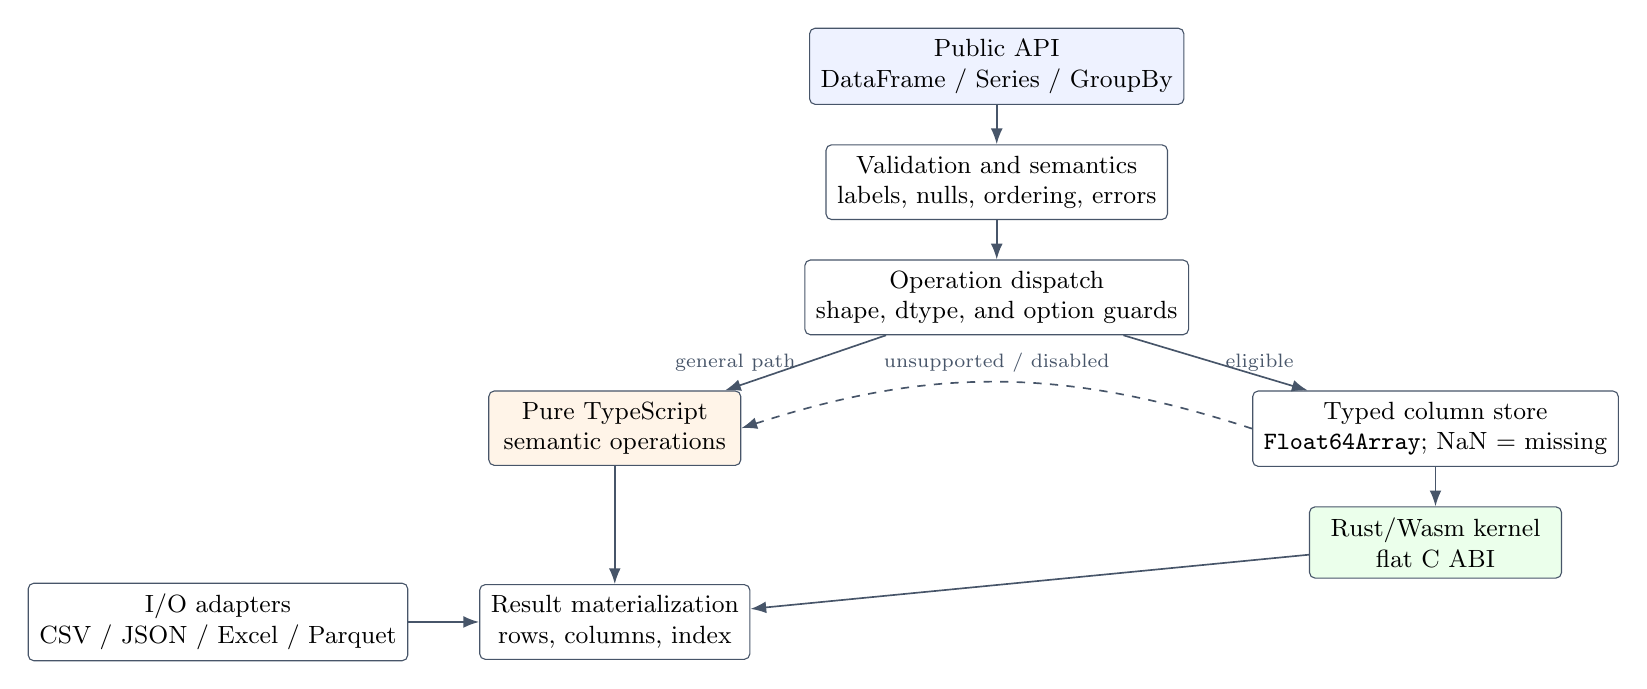
\begin{tikzpicture}[node distance=5mm and 9mm]
\node[layer, fill=bpink] (api) {Public API\\DataFrame / Series / GroupBy};
\node[layer, below=of api] (sem) {Validation and semantics\\labels, nulls, ordering, errors};
\node[layer, below=of sem] (dispatch) {Operation dispatch\\shape, dtype, and option guards};
\node[layer, below left=7mm and 8mm of dispatch, fill=orange!9] (ops) {Pure TypeScript\\semantic operations};
\node[layer, below right=7mm and 8mm of dispatch] (store) {Typed column store\\\texttt{Float64Array}; NaN = missing};
\node[layer, below=of store, fill=green!8] (wasm) {Rust/Wasm kernel\\flat C ABI};
\node[layer, below=15mm of ops] (materialize) {Result materialization\\rows, columns, index};
\node[layer, left=of materialize] (io) {I/O adapters\\CSV / JSON / Excel / Parquet};
\draw[flow] (api) -- (sem);
\draw[flow] (sem) -- (dispatch);
\draw[flow] (dispatch) -- node[left,note]{general path} (ops);
\draw[flow] (dispatch) -- node[right,note]{eligible} (store);
\draw[flow] (store) -- (wasm);
\draw[optional] (store.west) to[bend right=18] node[above,note]{unsupported / disabled} (ops.east);
\draw[flow] (ops) -- (materialize);
\draw[flow] (wasm) -- (materialize);
\draw[flow] (io) -- (materialize);
\end{tikzpicture}
}
\caption{Concrete architecture. Acceleration is a guarded branch inside an otherwise TypeScript execution path, not a second dataframe engine.}\label{fig:architecture}
\end{figure}

\subsection{Representation and semantic ownership}

Each DataFrame owns normalized rows, an ordered column list, and an index vector. This representation makes heterogeneous cells, label operations, and pandas-like row reconstruction straightforward, but numerical scans encounter object property access and boxed values. A weakly keyed column store builds only requested columns and reuses them while the row snapshot is unchanged. Finite numbers become contiguous \texttt{Float64Array} buffers; null and undefined become IEEE-754 NaN sentinels. Typed ingest primes isolated copies of numeric input, while in-place updates invalidate the store.

This cache does not make the library columnar. Every Wasm call still copies typed input into linear memory, and result rows still become JavaScript objects. Arrow defines a physical format for sharing buffers across languages \cite{arrowformat,dataframeprotocol}. \texttt{bun\_panda} does not yet use that representation and makes no zero-copy claim.

\subsection{Flat ABI and memory discipline}

The Rust module is built for \texttt{wasm32-unknown-unknown} without \texttt{wasm-bindgen}. Exports include allocation/reset functions, dense group-ID construction, single- and multi-plan floating-point aggregation, stable argsort, and filter-index compaction. Figure~\ref{fig:memory} shows the fused aggregation call. Plan-major output avoids one host call per reduction, but values, plan codes, group IDs, output, and counts still occupy separate contiguous regions.

\begin{figure}[t]
\centering
\resizebox{0.98\textwidth}{!}{%
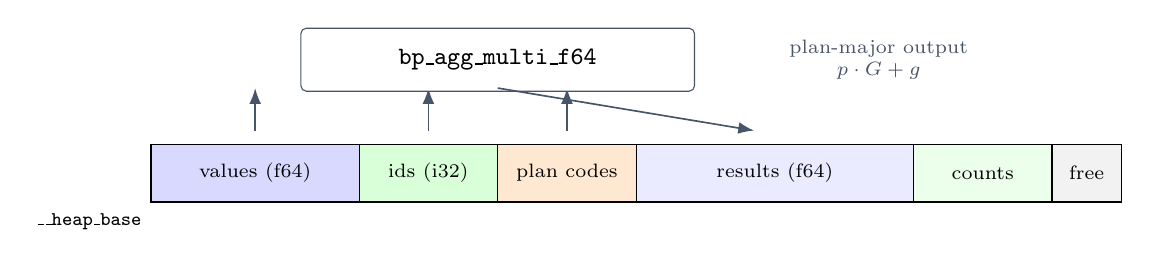
\begin{tikzpicture}[x=0.88cm,y=0.72cm]
\draw[thick] (0,0) rectangle (14,1);
\foreach \x/\w/\label/\col in {0/3/values (f64)/blue!15,3/2/ids (i32)/green!15,5/2/plan codes/orange!18,7/4/results (f64)/blue!8,11/2/counts/green!8,13/1/free/gray!10}{
  \fill[\col] (\x,0) rectangle ({\x+\w},1);
  \draw (\x,0) -- (\x,1);
  \node[font=\scriptsize,align=center] at ({\x+\w/2},0.5) {\label};
}
\draw (14,0) -- (14,1);
\node[anchor=east,font=\scriptsize] at (0,-0.35) {\texttt{\_\_heap\_base}};
\draw[flow] (1.5,1.25) -- (1.5,2.0);
\draw[flow] (4,1.25) -- (4,2.0);
\draw[flow] (6,1.25) -- (6,2.0);
\node[box,minimum width=50mm] at (5,2.5) {\texttt{bp\_agg\_multi\_f64}};
\draw[flow] (5,2.0) -- (8.7,1.25);
\node[note] at (10.5,2.5) {plan-major output\\$p\cdot G+g$};
\end{tikzpicture}
}
\caption{Wasm linear-memory layout for fused aggregation. The arena begins at the linker-exported heap base; every top-level call copies results before resetting the arena.}\label{fig:memory}
\end{figure}

During this study, a 250,000-row sequential-kernel test found that the original bump arena began at byte 8 rather than at the linker's exported \texttt{\_\_heap\_base}. Large allocations could overwrite static module data before memory growth. The corrected allocator starts at the linker symbol. A regression test now runs a 250,000-element argsort followed by mask compaction before performance data is accepted.

\subsection{Dispatch logic}

Figure~\ref{fig:dispatch} summarizes current dispatch. Correctness eligibility is checked before backend preference. The versioned calibration then considers operation, row count, requested top-$k$, and typed-column reuse. Named GroupBy requires \texttt{dropna=true}, supported reductions, and numeric plan columns. Sorting requires one numeric column and default missing-value placement. Filtering remains in TypeScript. \texttt{BUN\_PANDA\_WASM=0} forces TypeScript; \texttt{BUN\_PANDA\_WASM=1} forces only semantically eligible Wasm calls.

\begin{figure}[t]
\centering
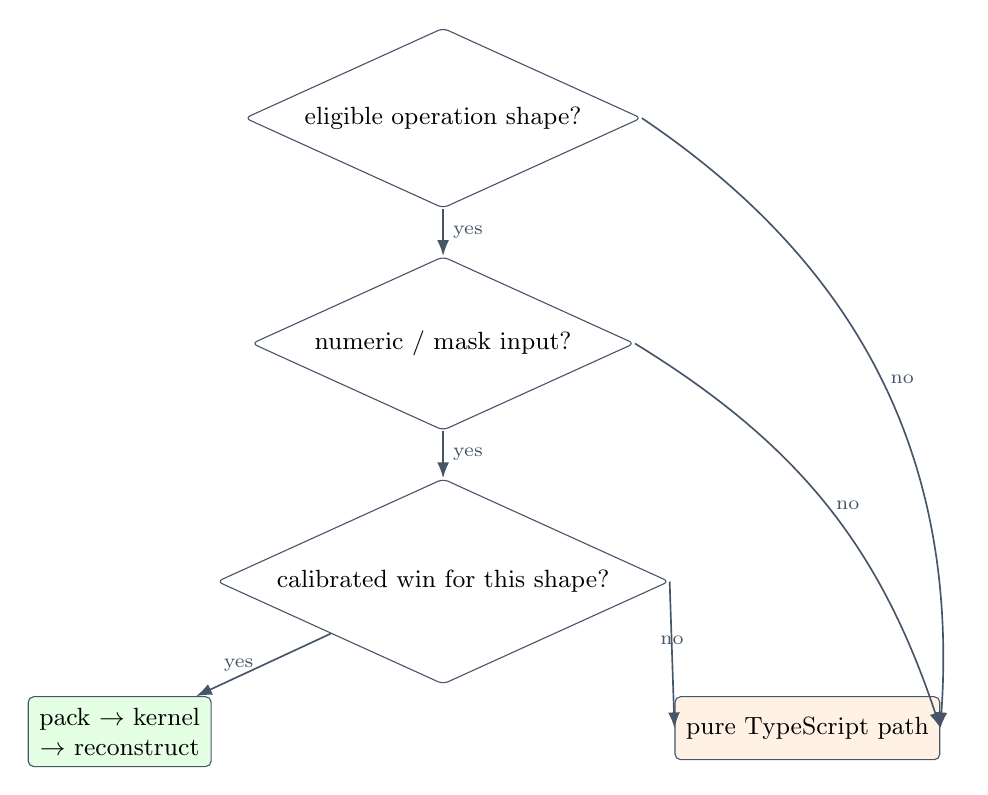
\begin{tikzpicture}[node distance=6mm and 10mm]
\node[box,diamond,aspect=2.2] (shape) {eligible operation shape?};
\node[box,diamond,aspect=2.2,below=of shape] (dtype) {numeric / mask input?};
\node[box,diamond,aspect=2.2,below=of dtype] (enabled) {calibrated win for this shape?};
\node[box,fill=green!10,below left=8mm and 15mm of enabled] (kernel) {pack $\rightarrow$ kernel\\$\rightarrow$ reconstruct};
\node[box,fill=orange!10,below right=8mm and 15mm of enabled] (ts) {pure TypeScript path};
\draw[flow] (shape) -- node[right,note]{yes} (dtype);
\draw[flow] (dtype) -- node[right,note]{yes} (enabled);
\draw[flow] (enabled) -- node[left,note]{yes} (kernel);
\draw[flow] (shape.east) to[bend left=30] node[right,note]{no} (ts.east);
\draw[flow] (dtype.east) to[bend left=20] node[right,note]{no} (ts.east);
\draw[flow] (enabled.east) -- node[above,note]{no} (ts.west);
\end{tikzpicture}
\caption{Correctness-first adaptive dispatch. Eligibility is necessary but does not imply that Wasm is profitable.}\label{fig:dispatch}
\end{figure}

\section{Compatibility and correctness method}\label{sec:compatibility}

\subsection{Name-level census}

The audit freezes four public groups from the pandas 3.0.5 documentation: 197 DataFrame methods and properties, 195 Series methods and properties, 75 top-level functions, and 38 GroupBy operations. A source extractor classifies each name as concrete, delegated, or intentionally unsupported and writes a machine-readable Markdown ledger. All \ApiCount{} names are present in version 0.4.0. The ledger exposes missing entry points. By itself, it says nothing about signatures, dtype fidelity, or edge cases.

\begin{figure}[t]
\centering
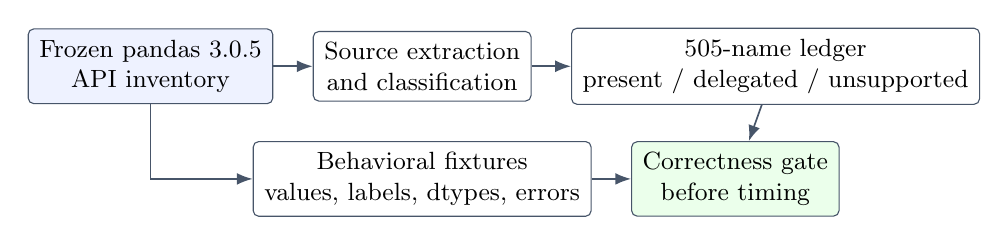
\begin{tikzpicture}[node distance=5mm]
\node[box,fill=bpink] (docs) {Frozen pandas 3.0.5\\API inventory};
\node[box,right=of docs] (extract) {Source extraction\\and classification};
\node[box,right=of extract] (ledger) {505-name ledger\\present / delegated / unsupported};
\node[box,below=of extract] (fixtures) {Behavioral fixtures\\values, labels, dtypes, errors};
\node[box,right=of fixtures,fill=green!8] (gate) {Correctness gate\\before timing};
\draw[flow] (docs) -- (extract);
\draw[flow] (extract) -- (ledger);
\draw[flow] (ledger) -- (gate);
\draw[flow] (docs) |- (fixtures);
\draw[flow] (fixtures) -- (gate);
\end{tikzpicture}
\caption{Compatibility evidence pipeline. Name coverage and behavioral agreement use different denominators and artifacts.}\label{fig:conformance}
\end{figure}

\subsection{Test oracle and failure handling}

The repository test suite uses deterministic fixtures for indexing, alignment, arithmetic, grouping, reshape, windows, I/O, and explicit error cases. The differential corpus adds 200 valid and 50 invalid or boundary cases for each of ten operation families. Both runtimes receive the same rows, column order, index labels, tagged non-finite values, operation, and arguments. The comparator checks status, output kind, values, labels, order, broad dtype families, exception categories, and input preservation. Null, NaN, NA, and NaT compare as the same missing mask; native dtype spellings remain in the raw artifact. For merges, the comparator requires the same sequence of join-key groups and the same row multiset within each contiguous equal-key group. It does not compare the internal pairing order of duplicate matches because pandas specifies preservation of left-key order, not duplicate-pair order \cite{pandas305}.

The corpus also runs \texttt{bun\_panda} with forced TypeScript, forced eligible Wasm, and adaptive dispatch. A backend mismatch aborts performance analysis for the corresponding input. The current \BackendPasses{}/\BackendCases{} backend agreement was reached after the oracle exposed an eligibility error: forced Wasm had routed \texttt{dropna=false} GroupBy through a kernel that always removes missing keys. Other oracle findings led to integer-period validation, missing-label validation in duplicate removal, corrected null ranking, and stable value-count tie order.

The adaptive implementation agrees with pandas in \ConformancePasses{} of \ConformanceCases{} observations under these declared comparison rules. This is \ConformancePercent{}\% of the tested corpus, not full pandas compatibility. MultiIndex, extension dtypes, warnings, categorical metadata, timezone semantics, and untested argument combinations remain outside the corpus.

\section{Experimental method}\label{sec:method}

\subsection{Research questions}

The evaluation asks: (RQ1) How closely does the tested semantic surface agree with pandas? (RQ2) Which eligible operations benefit from WebAssembly as input size grows? (RQ3) How does the system compare with four JavaScript, native, and WebAssembly alternatives under matched operation and load scopes? (RQ4) Do kernel-level conclusions transfer across browser engines? (RQ5) What distribution cost accompanies the design? (RQ6) Which failures point to changes in representation or dispatch?

\subsection{Environment}

Experiments ran on an Apple M5 Pro with 18 logical cores, 48 GiB RAM, and macOS 26.5. Versions were Bun 1.4.0, TypeScript 5.9.3, Rust 1.96.0, Arquero 8.0.3, Danfo.js 1.2.0, nodejs-polars 0.26.0, DuckDB-Wasm package 1.33.1-dev57.0 with embedded DuckDB 1.5.4, Python 3.13.13, and pandas 3.0.5. Browser measurements used headless Chromium \ChromiumVersion{}, Firefox \FirefoxVersion{}, and WebKit \WebkitVersion{} through Playwright. The benchmark process was single-threaded at the library level. Power mode and CPU frequency were not fixed. All host-level performance results in this manuscript are macOS measurements. Reports returned from Windows or Linux reproductions are reviewed as separate validation artifacts and are not pooled into these tables. The exact environment is stored in \texttt{paper/data/environment.json}.

\subsection{Datasets and matched operations}

The primary inputs use a deterministic linear congruential generator. The base schema contains numeric identifiers, values, weights, and revenue; categorical group, city, segment, and bucket strings; a boolean; and bounded-cardinality keys. Variants introduce skew, additional columns, unique keys, or periodic missing values. A public-data validation path uses the UCI Bank Marketing dataset, DOI \href{https://doi.org/10.24432/C5K306}{10.24432/C5K306}, under CC BY 4.0 \cite{ucibank}. The manifest fixes the source URL, archive and CSV SHA-256 digests, 45,211-row count, field mapping, and seed-independent transformations. Public-data correctness passed for every adapter; its timing is not mixed with the synthetic results.

The legacy Arquero comparison contains 82 cases: seven grouped reductions, 34 filtering, sorting, and top-$k$ pipelines, 32 counting variants, and nine joins. It remains useful as a broad exploratory profile. The principal cross-system study instead fixes four operations available in all five systems: grouped sum, filter then top-100 sort, value counts, and inner join. It runs at 10,000 and 50,000 rows under two scopes. The operation scope starts after each system has constructed its table. The load-plus-operation scope includes construction or registration but excludes process startup and package import. Each result is canonicalized to rows with explicit missing-value tags and compared by SHA-256 digest against a pure TypeScript reference.

\subsection{Timing protocol}

The legacy Arquero and pandas comparisons use three warm-up executions followed by eight measurements in each of three rounds. Their reported value is the median round mean, so these comparisons remain exploratory. The WebAssembly ablation uses fresh processes. Each workload, scale, backend, and replicate runs in a new Bun process. The controller randomizes all 720 tasks with a recorded seed. Each process constructs typed input, performs five warm-up calls, then records 20 calls. The final output is fully materialized and hashed with SHA-256. Inputs use paired seeds across backends, and all three digests must agree.

The experimental unit for the ablation is the process. For each effect, the analysis resamples processes and then iterations within the selected processes. It reports a 95\% hierarchical percentile bootstrap interval from 2,000 resamples \cite{georges2007statistically,kalibera2013rigorous}. A point estimate counts as a win only if the entire interval is above one. This design retains \FreshIterations{} iteration records nested inside \FreshProcesses{} processes. Warm-up can still be non-monotonic \cite{barrett2017warmup}.

The five-system study randomizes \CompetitorProcesses{} fresh process tasks. Each task performs three warm-ups and ten timed calls. Five process replicates cover every system, workload, scope, row count, and seed combination, yielding \CompetitorIterations{} timed calls across \CompetitorCells{} matched workload-scope-size cells. Reported values are medians of process means. The limited process count supports descriptive comparison, not confidence claims.

The browser study creates a new browser and dedicated module worker for every engine, scale, and replicate. The page is served with cross-origin isolation headers. Each worker instantiates the same WebAssembly asset, checks feature support, performs three warm-ups, and records ten TypeScript and ten WebAssembly calls for stable argsort, filter-index compaction, and grouped sum. Thirty replicates at 10,000 and 100,000 rows across three engines yield \BrowserContexts{} isolated contexts and \BrowserTimedCalls{} timed calls. Output hashes must match within every context. Browser speedup is the median across 30 context ratios at 100,000 rows. A deterministic 2,000-resample bootstrap over contexts supplies the reported 95\% intervals.

For ratios, define speedup as

\begin{equation}
S = \frac{T_{\mathrm{comparator}}}{T_{\mathrm{bun\_panda}}}.
\end{equation}

Thus $S>1$ favors \texttt{bun\_panda}. Aggregate speedups are geometric means of per-case ratios; unlike arithmetic means, this treats reciprocal slowdowns symmetrically.

\subsection{Package-size protocol}

The consumer tarball is measured with \texttt{npm pack --json --ignore-scripts} \cite{npmPack}. A minified Bun-target core bundle externalizes the optional \texttt{xlsx} and \texttt{parquetjs-lite} packages so that their independent cost is not attributed to core algorithms. A second build targets the browser-only kernel entry and rejects Node or Bun imports in its emitted graph. JavaScript and Wasm are reported raw, under gzip level 9, and under Brotli quality 11.

\section{Results}\label{sec:results}

\subsection{Behavioral conformance}

The 505-name census and the differential result answer different questions. The census records whether a name exists. The oracle finds \ConformancePasses{}/\ConformanceCases{} agreement against pandas 3.0.5 under the declared rules. All ten families agree in their 250 observations. The machine-readable summary records the numeric tolerance, dtype policy, and merge-order contract, while the mismatch ledger is empty for this corpus.

Forced TypeScript and forced eligible Wasm agree in \BackendPasses{}/\BackendCases{} observations, as do TypeScript and adaptive dispatch. This backend equality is a prerequisite for the timing study, not evidence of pandas compatibility.

\subsection{Exploratory Arquero profile}

Performance varies by workload family in Table~\ref{tab:arquero} and Figure~\ref{fig:families}. \texttt{bun\_panda} wins \ArqueroWins{} of \ArqueroCases{} cases, with an overall geometric-mean speedup of \ArqueroGeoSpeedup{}$\times$. Value-count workloads reach \CountsGeoSpeedup{}$\times$, and sort, filter, and top-$k$ workloads reach \SortGeoSpeedup{}$\times$. Group-by reaches \GroupbyGeoSpeedup{}$\times$. \texttt{bun\_panda} loses all nine merge cases; the family ratio of \MergeGeoSpeedup{}$\times$ means Arquero is approximately 2.92$\times$ faster there.

\begin{table}[t]
\caption{Arquero 8.0.3 comparison at 25,000 rows. Speedup is Arquero time divided by \texttt{bun\_panda} time.}\label{tab:arquero}
\begin{tabular}{@{}lrrrr@{}}
\toprule
Family & Cases & Wins & Losses & Geomean speedup \\
\midrule
Group-by & 7 & 6 & 1 & \GroupbyGeoSpeedup{}$\times$ \\
Sort/filter/top-$k$ & 34 & 34 & 0 & \SortGeoSpeedup{}$\times$ \\
Value counts & 32 & 32 & 0 & \CountsGeoSpeedup{}$\times$ \\
Merge/join & 9 & 0 & 9 & \MergeGeoSpeedup{}$\times$ \\
\midrule
Overall & \ArqueroCases{} & \ArqueroWins{} & 10 & \ArqueroGeoSpeedup{}$\times$ \\
\botrule
\end{tabular}
\end{table}

\begin{figure}[t]
\centering
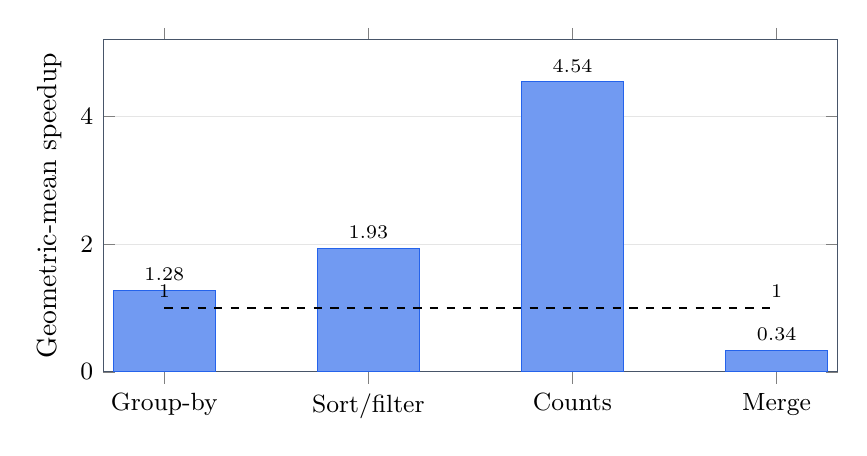
\begin{tikzpicture}
\begin{axis}[
  ybar, width=0.9\textwidth, height=58mm,
  ylabel={Geometric-mean speedup},
  symbolic x coords={Group-by,Sort/filter,Counts,Merge},
  xtick=data, ymin=0, ymax=5.2,
  bar width=13mm, nodes near coords,
  every node near coord/.append style={font=\scriptsize},
  axis line style={draw=bpgray}, tick label style={font=\small},
  ymajorgrids, grid style={gray!20}
]
\addplot[fill=bpblue!65,draw=bpblue] coordinates {
  (Group-by,\GroupbyGeoSpeedup) (Sort/filter,\SortGeoSpeedup)
  (Counts,\CountsGeoSpeedup) (Merge,\MergeGeoSpeedup)};
\addplot[sharp plot,thick,dashed,black] coordinates {(Group-by,1) (Merge,1)};
\end{axis}
\end{tikzpicture}
\caption{Family-level performance against Arquero. The dashed line marks parity. Complete per-case values are retained in the JSON artifact.}\label{fig:families}
\end{figure}

The implementation choices explain much of this spread. Bounded value counts avoid a general relational plan, and top-$k$ selection can avoid a full multi-column sort. Merge creates and copies row objects, resolves colliding names, and materializes wide results. Arquero's column-oriented join path suits that workload better. Faster joins will require changes to representation and materialization rather than another arithmetic kernel.

\subsection{Exploratory pandas profile}

Across ten matched cases, \texttt{bun\_panda} wins \PandasWins{} and loses four, with a \PandasGeoSpeedup{}$\times$ geometric-mean speedup. Table~\ref{tab:pandas} gives all cases because the sample is small. The largest advantage is high-cardinality single-key value counts (0.27$\times$ time ratio, or 3.73$\times$ speedup); the largest disadvantage is single-column top-1000 sorting (2.33$\times$ slower). Multi-column top-800 sorting is effectively tied.

\begin{table}[t]
\caption{Matched pandas 3.0.5 comparison at 25,000 rows. Ratio below 1 favors \texttt{bun\_panda}.}\label{tab:pandas}
\begin{tabular}{@{}lrrr@{}}
\toprule
Case & bun\_panda (ms) & pandas (ms) & bun/pandas \\
\midrule
groupby mean & 4.67 & 3.78 & 1.23 \\
filter + sort top 100 & 1.42 & 2.99 & 0.48 \\
sort top 1000 & 5.07 & 2.17 & 2.33 \\
multi-column sort top 800 & 10.44 & 10.43 & 1.00 \\
value counts: city & 0.74 & 3.20 & 0.23 \\
value counts: group/city top 10 & 2.50 & 5.89 & 0.43 \\
missing city, retain null & 0.91 & 1.39 & 0.66 \\
missing city group-by mean & 2.71 & 3.16 & 0.86 \\
high-cardinality city top 20 & 20.04 & 15.18 & 1.32 \\
high-cardinality user top 100 & 9.08 & 33.90 & 0.27 \\
\botrule
\end{tabular}
\end{table}

This is a cross-runtime comparison between Bun/JavaScriptCore and CPython/native pandas extensions. It does not isolate language, runtime, data representation, or implementation. pandas remains the semantic reference; these timings answer only whether the selected operation completes faster under the stated environment.

\subsection{Matched five-system study (RQ3)}

Table~\ref{tab:competitor-operation} reports operation-only medians at 50,000 rows. \texttt{bun\_panda} is faster than Arquero, Danfo.js, and DuckDB-Wasm on grouped sum, filter plus top-100 sort, and value counts. nodejs-polars is faster on grouped sum and filtering. The ranking reverses for join: \texttt{bun\_panda} needs \JoinBunPandaOpMs{} ms, compared with \JoinPolarsOpMs{} ms for nodejs-polars, \JoinArqueroOpMs{} ms for Arquero, and \JoinDuckDBOpMs{} ms for DuckDB-Wasm. Danfo.js is slower on all four cells in this environment.

\begin{table}[t]
\caption{Operation-only median of process means at 50,000 rows, in milliseconds. Lower is better. Each cell contains five fresh processes and 50 timed calls.}\label{tab:competitor-operation}
\centering
\small
\setlength{\tabcolsep}{4pt}
\begin{tabular}{@{}lrrrrr@{}}
\toprule
Workload & bun\_panda & Arquero & Danfo.js & nodejs-polars & DuckDB-Wasm \\
\midrule
Grouped sum & \GroupBunPandaOpMs & \GroupArqueroOpMs & \GroupDanfoOpMs & \GroupPolarsOpMs & \GroupDuckDBOpMs \\
Filter and top-100 sort & \FilterBunPandaOpMs & \FilterArqueroOpMs & \FilterDanfoOpMs & \FilterPolarsOpMs & \FilterDuckDBOpMs \\
Value counts & \CountsBunPandaOpMs & \CountsArqueroOpMs & \CountsDanfoOpMs & \CountsPolarsOpMs & \CountsDuckDBOpMs \\
Inner join & \JoinBunPandaOpMs & \JoinArqueroOpMs & \JoinDanfoOpMs & \JoinPolarsOpMs & \JoinDuckDBOpMs \\
\bottomrule
\end{tabular}
\end{table}

Load-plus-operation timing in Table~\ref{tab:competitor-load} changes the interpretation. \texttt{bun\_panda}, Arquero, and nodejs-polars are close on grouped sum and filtering. DuckDB-Wasm pays about 118 to 126 ms per measured construction and query because the scope includes table registration in a fresh embedded database connection, though not module import or process startup. This is a deliberately literal application boundary, not an estimate of a long-lived DuckDB session. The paired tables show why a single headline speedup would be misleading.

\begin{table}[t]
\caption{Load-plus-operation median of process means at 50,000 rows, in milliseconds. Lower is better.}\label{tab:competitor-load}
\centering
\small
\setlength{\tabcolsep}{4pt}
\begin{tabular}{@{}lrrrrr@{}}
\toprule
Workload & bun\_panda & Arquero & Danfo.js & nodejs-polars & DuckDB-Wasm \\
\midrule
Grouped sum & \GroupBunPandaLoadMs & \GroupArqueroLoadMs & \GroupDanfoLoadMs & \GroupPolarsLoadMs & \GroupDuckDBLoadMs \\
Filter and top-100 sort & \FilterBunPandaLoadMs & \FilterArqueroLoadMs & \FilterDanfoLoadMs & \FilterPolarsLoadMs & \FilterDuckDBLoadMs \\
Value counts & \CountsBunPandaLoadMs & \CountsArqueroLoadMs & \CountsDanfoLoadMs & \CountsPolarsLoadMs & \CountsDuckDBLoadMs \\
Inner join & \JoinBunPandaLoadMs & \JoinArqueroLoadMs & \JoinDanfoLoadMs & \JoinPolarsLoadMs & \JoinDuckDBLoadMs \\
\bottomrule
\end{tabular}
\end{table}

All \CompetitorCells{} matched workload-scope-size cells pass the digest gate for all five systems. The study does not claim semantic equivalence outside those four operations. It also avoids averaging incompatible workloads into one score.

The checksum-pinned UCI workload adds \PublicProcesses{} fresh processes and \PublicIterations{} timed calls across \PublicCells{} matched cells. Table~\ref{tab:public-operation} shows that the synthetic ranking is not universal. At 45,211 public rows, nodejs-polars leads grouped sum, filtering, and value counts, while Arquero leads join narrowly ahead of DuckDB-Wasm. \texttt{bun\_panda} does not lead an operation-only cell, although it remains faster than Arquero on filtering and value counts. Its join time widens to \PublicJoinBunPandaOpMs{} ms versus \PublicJoinArqueroOpMs{} ms for Arquero. In load-plus-operation scope, \texttt{bun\_panda} records \PublicCountsBunPandaLoadMs{} ms for value counts, lower than all four alternatives, while DuckDB-Wasm again pays per-call registration cost. This public-data reversal is evidence against a library-wide performance claim.

\begin{table}[t]
\caption{Operation-only median of process means on the 45,211-row UCI Bank Marketing workload, in milliseconds. Lower is better.}\label{tab:public-operation}
\centering
\small
\setlength{\tabcolsep}{4pt}
\begin{tabular}{@{}lrrrrr@{}}
\toprule
Workload & bun\_panda & Arquero & Danfo.js & nodejs-polars & DuckDB-Wasm \\
\midrule
Grouped sum & \PublicGroupBunPandaOpMs & \PublicGroupArqueroOpMs & \PublicGroupDanfoOpMs & \PublicGroupPolarsOpMs & \PublicGroupDuckDBOpMs \\
Filter and top-100 sort & \PublicFilterBunPandaOpMs & \PublicFilterArqueroOpMs & \PublicFilterDanfoOpMs & \PublicFilterPolarsOpMs & \PublicFilterDuckDBOpMs \\
Value counts & \PublicCountsBunPandaOpMs & \PublicCountsArqueroOpMs & \PublicCountsDanfoOpMs & \PublicCountsPolarsOpMs & \PublicCountsDuckDBOpMs \\
Inner join & \PublicJoinBunPandaOpMs & \PublicJoinArqueroOpMs & \PublicJoinDanfoOpMs & \PublicJoinPolarsOpMs & \PublicJoinDuckDBOpMs \\
\bottomrule
\end{tabular}
\end{table}

\subsection{WebAssembly ablation (RQ2)}

Table~\ref{tab:fresh-wasm} reports the fresh-process ablation. The effect is mean TypeScript time divided by mean candidate time. Full numeric sorting and fused four-plan GroupBy over reused typed columns win at every scale. Top-1,000 selection wins at 10,000 rows, but both larger intervals cross one. Forced Wasm filtering loses by a wide margin. Adaptive filtering stays in TypeScript, so its intervals center near parity and remain unresolved.

\begin{table}[t]
\caption{Fresh-process speedups with 95\% hierarchical bootstrap intervals. Each cell has 20 processes and 20 measured calls per process.}\label{tab:fresh-wasm}
\begin{tabular}{@{}lrrl@{}}
\toprule
Workload & Rows & Forced Wasm [95\% CI] & Verdict \\
\midrule
Fused GroupBy, 4 plans & 10,000 & 1.523 [1.069, 2.306] & win \\
 & 100,000 & 1.442 [1.285, 1.642] & win \\
 & 250,000 & 1.599 [1.323, 1.903] & win \\
Full numeric sort & 10,000 & 1.713 [1.471, 1.983] & win \\
 & 100,000 & 1.669 [1.298, 2.087] & win \\
 & 250,000 & 1.752 [1.370, 2.186] & win \\
Top-1,000 sort & 10,000 & 1.458 [1.182, 1.744] & win \\
 & 100,000 & 0.901 [0.737, 1.081] & unresolved \\
 & 250,000 & 0.869 [0.594, 1.258] & unresolved \\
Boolean-mask filter & 10,000 & 0.199 [0.163, 0.241] & loss \\
 & 100,000 & 0.547 [0.459, 0.651] & loss \\
 & 250,000 & 0.308 [0.269, 0.358] & loss \\
\botrule
\end{tabular}
\end{table}

The resulting calibration is conservative. Full numeric sort uses Wasm from 10,000 rows. Fused GroupBy uses Wasm from 10,000 rows only when every plan column is already cached and \texttt{dropna=true}. Top-1,000 uses Wasm only at the measured 10,000-row boundary; larger inputs use bounded TypeScript selection. Filtering stays in TypeScript. The environment override can force eligible Wasm calls for experiments, but it cannot bypass semantic eligibility.

\subsection{Cross-engine browser execution (RQ4)}

All three engines provide WebAssembly, streaming instantiation, threads, SIMD, shared memory, and cross-origin isolation in the tested build. WebKit reports no relaxed SIMD support. Median initialization is \ChromiumInitMs{} ms in Chromium, \FirefoxInitMs{} ms in Firefox, and \WebkitInitMs{} ms in WebKit. This one-time cost is excluded from the warm kernel ratios in Table~\ref{tab:browser}.

\begin{table}[t]
\caption{Median TypeScript-time divided by WebAssembly-time ratio at 100,000 rows across 30 isolated contexts per engine, with 95\% bootstrap intervals. Values above 1 favor WebAssembly.}\label{tab:browser}
\centering
\small
\setlength{\tabcolsep}{4pt}
\begin{tabular}{@{}lrrr@{}}
\toprule
Engine & Stable argsort & Filter indices & Grouped sum \\
\midrule
Chromium & \ChromiumSortSpeedup{} [\ChromiumSortLower, \ChromiumSortUpper] & \ChromiumFilterSpeedup{} [\ChromiumFilterLower, \ChromiumFilterUpper] & \ChromiumGroupSpeedup{} [\ChromiumGroupLower, \ChromiumGroupUpper] \\
Firefox & \FirefoxSortSpeedup{} [\FirefoxSortLower, \FirefoxSortUpper] & \FirefoxFilterSpeedup{} [\FirefoxFilterLower, \FirefoxFilterUpper] & \FirefoxGroupSpeedup{} [\FirefoxGroupLower, \FirefoxGroupUpper] \\
WebKit & \WebkitSortSpeedup{} [\WebkitSortLower, \WebkitSortUpper] & \WebkitFilterSpeedup{} [\WebkitFilterLower, \WebkitFilterUpper] & \WebkitGroupSpeedup{} [\WebkitGroupLower, \WebkitGroupUpper] \\
\bottomrule
\end{tabular}
\end{table}

\begin{figure}[t]
\centering
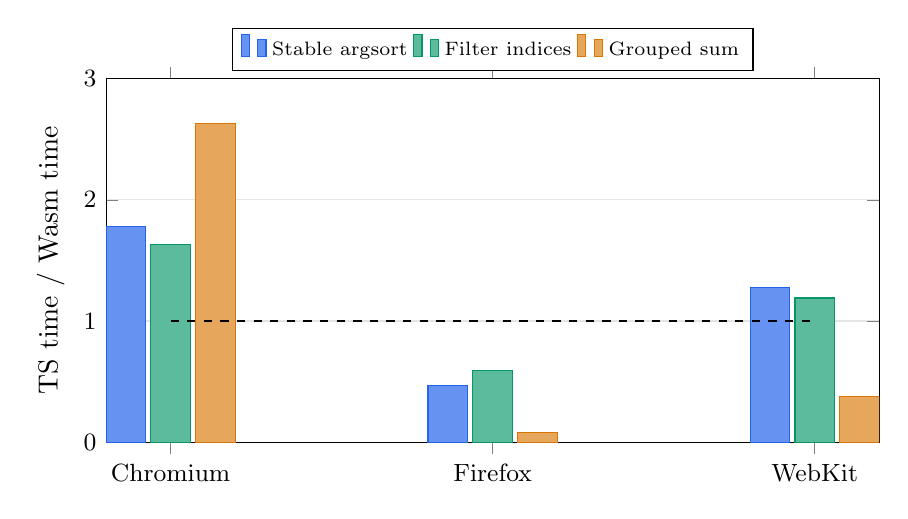
\begin{tikzpicture}
\begin{axis}[
  ybar, width=0.94\textwidth, height=62mm,
  ylabel={TS time / Wasm time},
  symbolic x coords={Chromium,Firefox,WebKit}, xtick=data,
  ymin=0, ymax=3.0, bar width=5mm,
  legend style={at={(0.5,1.02)},anchor=south,legend columns=3,font=\scriptsize},
  ymajorgrids, grid style={gray!20}, tick label style={font=\small}
]
\addplot[fill=bpblue!70,draw=bpblue] coordinates {(Chromium,\ChromiumSortSpeedup) (Firefox,\FirefoxSortSpeedup) (WebKit,\WebkitSortSpeedup)};
\addplot[fill=bpgreen!65,draw=bpgreen] coordinates {(Chromium,\ChromiumFilterSpeedup) (Firefox,\FirefoxFilterSpeedup) (WebKit,\WebkitFilterSpeedup)};
\addplot[fill=bporange!65,draw=bporange] coordinates {(Chromium,\ChromiumGroupSpeedup) (Firefox,\FirefoxGroupSpeedup) (WebKit,\WebkitGroupSpeedup)};
\addplot[sharp plot,thick,dashed,black] coordinates {(Chromium,1) (WebKit,1)};
\legend{Stable argsort,Filter indices,Grouped sum}
\end{axis}
\end{tikzpicture}
\caption{Browser kernel ratios at 100,000 rows. The dashed parity line exposes the engine-dependent reversal.}\label{fig:browser}
\end{figure}

The browser result is not a full DataFrame benchmark. It isolates typed numeric kernels in a dedicated worker and therefore answers whether an already-eligible kernel transfers across engines. It does not include row-object conversion or network download. Even at that favorable boundary, Firefox reverses every conclusion, and WebKit reverses grouped sum. Runtime identity must therefore be part of any browser dispatch calibration.

\subsection{Package and bundle size (RQ5)}

The npm tarball is \NpmTarballKiB{} KiB and expands to \NpmUnpackedKiB{} KiB across \NpmEntryCount{} entries. The minified full core bundle, with optional Excel and Parquet dependencies externalized, is \CoreBundleKiB{} KiB raw and \CoreBundleGzipKiB{} KiB under gzip. The browser kernel entry is \BrowserBundleBytes{} bytes raw, \BrowserBundleGzipBytes{} bytes under gzip, and \BrowserBundleBrotliBytes{} bytes under Brotli. The separate \WasmBytes{}-byte module compresses to \WasmGzipBytes{} and \WasmBrotliBytes{} bytes, respectively.

\begin{center}
\centering
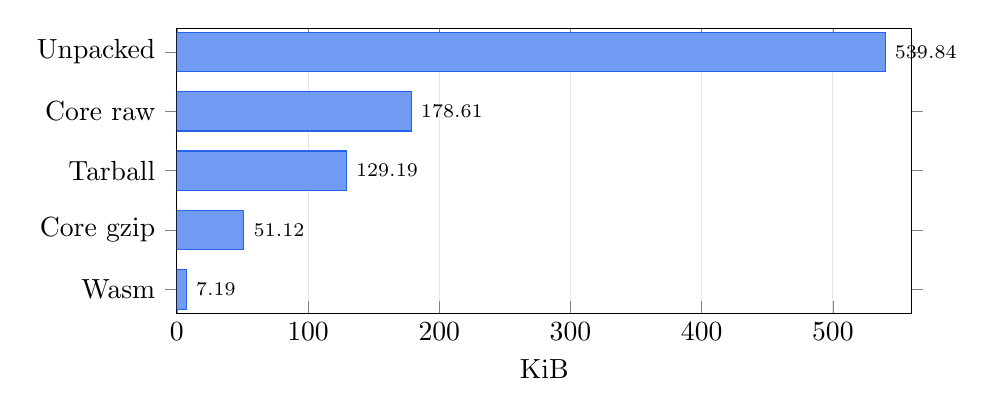
\begin{tikzpicture}
\begin{axis}[
  xbar, width=0.9\textwidth,height=52mm,
  xlabel={KiB}, symbolic y coords={Wasm,Core gzip,Tarball,Core raw,Unpacked},
  ytick=data, xmin=0, xmax=560, nodes near coords,
  every node near coord/.append style={font=\scriptsize},
  xmajorgrids,grid style={gray!20}, bar width=5mm
]
\addplot[fill=bpblue!65,draw=bpblue] coordinates {
 (7.19,Wasm) (51.12,Core gzip) (129.19,Tarball)
 (178.61,Core raw) (539.84,Unpacked)};
\end{axis}
\end{tikzpicture}
\captionof{figure}{Distinct distribution artifacts. The scales are not interchangeable: the tarball includes source files, while the core bundle externalizes optional I/O packages.}\label{fig:size}
\end{center}

The full Bun loader reads and instantiates WebAssembly synchronously on the first eligible call. The browser entry has a different contract: it uses \texttt{instantiateStreaming(fetch(url))}, falls back to asynchronous byte instantiation when the server sends the wrong MIME type, and accepts preloaded bytes for workers or offline bundles. Static graph checks, byte-level kernel tests, and the three-engine worker study all pass.

\section{Discussion}\label{sec:discussion}

\subsection{Architectural findings}

Conversion cost matters more than the kernel language in several cases. The same 7.2 KiB module produces a 1.71$\times$ full-sort point speedup and a fivefold slowdown for a 10,000-row filter in Bun. Mask compaction is a linear JavaScript loop, and its output still requires JavaScript row gathering. A small Rust loop does not recover the cost of two copies and a host call.

Runtime implementation also matters. At 100,000 rows, stable argsort favors WebAssembly in Chromium and WebKit but loses in Firefox. Grouped sum ranges from 2.56$\times$ in Chromium to 0.08$\times$ in Firefox. These tests use the same bytes, inputs, worker boundary, warm-up rule, and digest gate. A calibration learned from Bun or Chromium is therefore not portable evidence for another engine.

Algorithm choice explains the 250,000-row top-1000 reversal. The Wasm path performs a full stable argsort. A bounded heap or selection algorithm would change the work from $O(n\log n)$ toward $O(n\log k)$, but moving that algorithm to Wasm would not guarantee a faster result. Dispatch must consider the requested operation, not only dtype.

Row-oriented storage has a visible join cost. A merge produces new heterogeneous row objects and resolves colliding column names. Numeric Wasm kernels do not reduce that materialization work. Columnar join indices could postpone row reconstruction, but they would also enlarge the semantic core and require additional label and null tests.

The 505-name census creates a large testing obligation. The generated oracle covers ten families and found implementation defects even though only one of 2,500 observations now differs from pandas. The result applies to this corpus, not to untested extension dtypes, time zones, categorical metadata, warnings, or copy-on-write behavior. Adding names is cheap compared with specifying and testing those semantics.

\subsection{Revised dispatch policy}

Table~\ref{tab:policy} states the default supported by each measured result.

\begin{center}
\captionof{table}{Dispatch changes supported by the measured ablation.}\label{tab:policy}
\small
\begin{tabularx}{\textwidth}{@{}p{28mm}Xp{38mm}@{}}
\toprule
Operation & Recommendation & Evidence \\
\midrule
Full numeric sort & Use Wasm from 10,000 rows & Every measured interval is above one \\
Top-$k$ numeric sort & Use Wasm only at the measured 10,000-row cell & Larger intervals cross one \\
Boolean mask & Keep TypeScript default & Every forced-Wasm interval is below one \\
Fused numeric group-by & Use Wasm when typed plan columns are cached & Every reused-column interval is above one \\
Merge/join & Optimize representation, not arithmetic kernel & 0/9 wins vs Arquero \\
Browser kernels & Calibrate independently for each engine and version & Ratios reverse across Chromium, Firefox, and WebKit \\
\botrule
\end{tabularx}
\end{center}

\subsection{Interoperability roadmap}

Parquet support passes through \texttt{parquetjs-lite}. It provides file interoperability, not an Arrow-native or zero-copy data path. Parquet organizes storage into row groups, column chunks, and pages with defined encodings and compression \cite{parquetformat}. Arrow defines a language-independent in-memory layout \cite{arrowformat}. An optional columnar backend could share buffers among Parquet decoding, dataframe operations, and Wasm when alignment and ownership permit. Any zero-copy claim would first require buffer-identity and allocation measurements.

\section{Threats to validity}\label{sec:threats}

\textbf{Construct validity.} The comparisons emphasize operations implemented by every participant and do not represent the entire dataframe task distribution. Canonical output hashing forces result materialization but does not serialize every result into an external format. The 505-name metric measures discoverability, not semantic compatibility. The browser study measures typed kernels, not the full DataFrame API. Package-size measurements externalize optional I/O dependencies and are not a full application bundle.

\textbf{Internal validity.} The main ablation and five-system study use fresh processes and randomized order, but they still run on an interactive workstation without fixed frequency, thermal, or power controls. Fixed warm-up counts are protocol choices rather than proof of steady state. Browser ratios have 30 independent contexts per engine and scale. The legacy Arquero and pandas timing tables remain single-process exploratory results.

\textbf{External validity.} Host-level results come from one Apple M5 Pro and Bun 1.4.0. They may not transfer to x86-64 Linux, different JavaScriptCore revisions, larger-than-memory data, or string-heavy workloads. The browser study broadens engine coverage but shares the same arm64 host. The compared systems have different semantics and representations; only the listed operations are matched.

\textbf{Conclusion validity.} The ablation intervals resample processes and iterations, and every timed backend passes a paired output digest. Browser intervals resample 30 independent contexts, while the five-system tables remain descriptive because their five-process replication is too small for strong interval claims. No result establishes a universal speedup. Native x86-64 replication and controlled Linux cgroup measurements would strengthen transferability and capacity analysis, but neither is part of the present result set.

\section{Reproducibility and artifact}\label{sec:artifact}

The repository includes the official December 2024 Springer Nature template archive with its SHA-256 digest, unmodified template sources, the manuscript, benchmark scripts, raw JSON samples, environment capture, package analysis, generated macros, a checksum-pinned public workload manifest, and Linux runners. Figure~\ref{fig:evidence} shows how raw evidence reaches manuscript claims.

\begin{figure}[t]
\centering
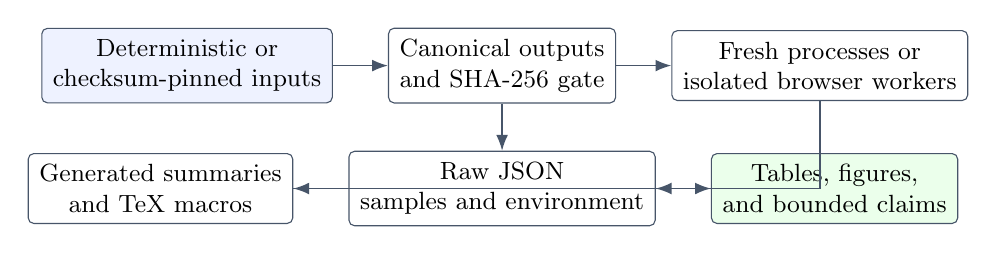
\begin{tikzpicture}[node distance=6mm and 7mm]
\node[box,fill=bpink] (inputs) {Deterministic or\\checksum-pinned inputs};
\node[box,right=of inputs] (gate) {Canonical outputs\\and SHA-256 gate};
\node[box,right=of gate] (runs) {Fresh processes or\\isolated browser workers};
\node[box,below=of gate] (raw) {Raw JSON\\samples and environment};
\node[box,left=of raw] (summary) {Generated summaries\\and TeX macros};
\node[box,right=of raw,fill=green!8] (claims) {Tables, figures,\\and bounded claims};
\draw[flow] (inputs) -- (gate);
\draw[flow] (gate) -- (runs);
\draw[flow] (runs) |- (raw);
\draw[flow] (gate) -- (raw);
\draw[flow] (raw) -- (summary);
\draw[flow] (summary) -- (claims);
\end{tikzpicture}
\caption{Evidence path. A timing is reportable only after its output passes the reference digest and its raw record retains the execution context.}\label{fig:evidence}
\end{figure}

The minimal local reproduction sequence is:

\begin{lstlisting}[language=bash]
bun install
bun run build:wasm
bun test
bun run conformance
bun run bench:fresh
bun run bench:competitors
bun run bench:browser
bun run workload:public
bun run bench:competitors:uci
bun run paper/artifact/analyze-package-size.ts
bun run paper/artifact/summarize-study.ts
bun run paper/artifact/summarize-expanded-study.ts
bun run artifact:checksums
\end{lstlisting}

The repository also includes an optional x86-64 route that builds a digest-pinned \texttt{linux/amd64} container and refuses to label a run as native unless \texttt{uname -m} reports \texttt{x86\_64}. A separate cgroup runner can apply the same memory and memory-swap limit to each system, record current and peak memory, capture memory events, and report out-of-memory termination. Apple-hosted instruction emulation was rejected after Bun faulted under an emulated CPU lacking AVX; no emulated timing appears in the results. A separate cross-platform runner executes the correctness, package, conformance, host, public-data, and browser studies on macOS, Windows, or Linux and embeds their outputs in one returnable JSON report.

Raw artifacts retain every fresh-process iteration, correctness digest, process diagnostic, differential observation, mismatch category, and rejected-run reason. The repository includes commands for every reported measurement and follows the documentation, consistency, completeness, and exerciseability criteria used in artifact review \cite{acmartifact}. A versioned archival DOI and independent clean-checkout reproduction remain pre-submission tasks. Cross-platform timing reports will remain separate from the macOS tables unless a later revision defines and executes a multi-host design.

\section{Conclusion}\label{sec:conclusion}

\texttt{bun\_panda} combines pandas-inspired TypeScript semantics with a small Rust/WebAssembly kernel set. The differential oracle reaches \ConformancePercent{}\% agreement in the tested ten-family corpus under its declared value, label, dtype, exception, mutation, and ordering rules. The fresh-process ablation supports WebAssembly for full numeric sort and fused GroupBy over cached typed columns, but not for mask filtering or large top-1,000 selection. The five-system study finds favorable synthetic counting and filtering cells, no public operation-only win, and a persistent join deficit. The browser study then shows that even typed-kernel conclusions reverse across engines. Backend selection must account for semantics, operation shape, representation reuse, and runtime version. The current evidence package therefore makes macOS-scoped performance claims; cross-platform replication and controlled capacity measurement remain future validation work.

\backmatter

\bmhead{Acknowledgements}
N/A.

\bmhead{Author contributions}
Touhidul Alam Seyam is the sole author of the current manuscript.

\bmhead{Funding}
N/A.

\bmhead{Data availability}
Primary benchmark inputs are generated deterministically by scripts included in the artifact. The optional public-data validation uses the UCI Bank Marketing dataset under CC BY 4.0. Its DOI, source URL, field mapping, row count, and SHA-256 checksums are fixed in the workload manifest. No private dataset is required.

\bmhead{Code availability}
Source, raw measurements, and reproduction scripts are available in the immutable \href{https://github.com/Seyamalam/bun_panda/releases/tag/v0.4.1}{GitHub release v0.4.1}. The corresponding software package is available from \href{https://www.npmjs.com/package/bun_panda/v/0.4.1}{npm as bun\_panda 0.4.1}. The experiments report version 0.4.0 because that is the version recorded in the frozen raw measurements; version 0.4.1 packages the same evaluated implementation with the paper artifact and release metadata. A persistent archival identifier will be added before submission.

\bmhead{Conflict of interest}
None.

\renewcommand{\bibfont}{\small}
\setlength{\bibsep}{0.5em}
\bibliography{references}

\end{document}
